\section{Anforderungen}

Die Anforderungsanalyse spezifiziert die Anforderungen an das
Browser Shape Tool. 
Mithilfe einer Recherche und Brainstorming werden die Nutzungsanforderungen
aufgestellt und daraus die funktionalen und nicht-funktionalen
Anforderungen abgeleitet. Grafische Entwürfe der Benutzeroberfläche
werden zeigen, wie die Nutzungsanforderungen aus Blackbox-Sicht
umgesetzt werden können.

\paragraph{Projektvorgaben}
Nachstehend sind die Vorgaben der Projektaufttraggeber definiert:
\begin{itemize}
  \item Implementation eines JS-Browser-Frameworks,
  \item Spray Definition annehmen, verarbeiten, interpretieren, darstellen,
  \item Darstellung ist Eclipse Graphiti-like,
  \item Shape-Darstellungen bearbeiten können,
  \item Diagramm-Modell muss validierbar und persistierbar sein.
\end{itemize}

\subsection{Nutzungsanforderungen}
Um die Funktionen des Systems zu definieren, müssen zuerst die Nutzungsanforderungen
identifiziert werden. Diese sind sogenannte Akzeptanzkriterien und werden
im Abnahmetest, welcher am Ende des Projekts durchgeführt wird, validiert.
Auf Tabelle \ref{tbl.nutz} werden die Nutzungsanforderungen gelistet,
nummeriert und nach dem MoSCoW-Prinzip priorisiert:

\begin{itemize}
  \item Must  (M, unbedingt erforderlich)
  \item Should (S, sollte umgesetzt werden)
  \item Could (C, kann umgesetzt werden)
  \item Won’t (W, wird nicht umgesetzt, aber für die Zukunft vorgemerkt)
\end{itemize}

\begin{table}[tbp]
  \begin{tabular}{ | c | p{10cm} | c | }
    \hline
    \# & Anforderung & Prio. \\ \hline \hline
    1  & Der Nutzer muss das Modell betrachten können. & C \\ \hline
    2  & Der Nutzer muss das Modell z.B. als Dokumentation einbinden können. (d.h. der View Mode muss druckbar seitens eines Webbrowsers sein). & C \\ \hline
    3  & Der Nutzer muss das Modell bearbeiten können. & M \\ \hline
    4  & Das System muss eine Spray Shape Definition laden können. & M \\ \hline
    5  & Das System muss die Semantik eines Shapes verstehen/abbilden können. & M \\ \hline
    6  & Der Nutzer muss Shape-Elemente gemäß der zugrunde liegenden Spray Shape-DSL zeichnen können. Der Nutzer muss eine Aufzählung, Auswahl bzw. Übersicht aller ermöglichten Shape-Elemente erhalten. & M \\ \hline
    7  & Der Nutzer muss die Bearbeitungssicht zoomen können. & C \\ \hline
    8  & Der Nutzer muss den Zustand speichern können. (i) Koordinaten eines jeden Elements, (ii) Das eigentliche (semantische) Modell. & M \\ \hline
    9 & Der Nutzer muss einen gespeicherten Zustand des Modells laden können.
(i) Koordinaten eines jeden Elements, (ii)
das eigentliche (semantische) Modell. & M \\ \hline
    10 & Der Nutzer muss erkennen können, ob der Zustand valide ist oder nicht. & C \\ \hline
    11 & Der Nutzer muss durch das System die Elemente automatisch ausrichten lassen können. „Ausrichtungsassistenz“ & W \\
    \hline  
  \end{tabular}
  \caption{Nutzungsanforderungen für Spray Web,
           nach dem MoSCoW-Prinzip priorisiert.}\label{tbl.nutz}
\end{table}

\subsection{Funktionale Anforderungen}\label{sec.funcAnforderung}

Anhand von grafischen Entwürfen (siehe Abbildung
\ref{fig.gui} und \ref{fig.guiAnker}) der Benutzeroberfläche wird dargestellt,
wie die Nutzungsanforderungen aus Blackbox-Sicht umgesetzt werden sollen.
Die Screens und die dazugehörigen Beschreibungen definieren, wie das Shape-Tool 
funktioniert und wie es zu bedienen ist. Diese Systemanforderungen werden
im Systemtest verifiziert.

\begin{figure}[h!]
  \centering
  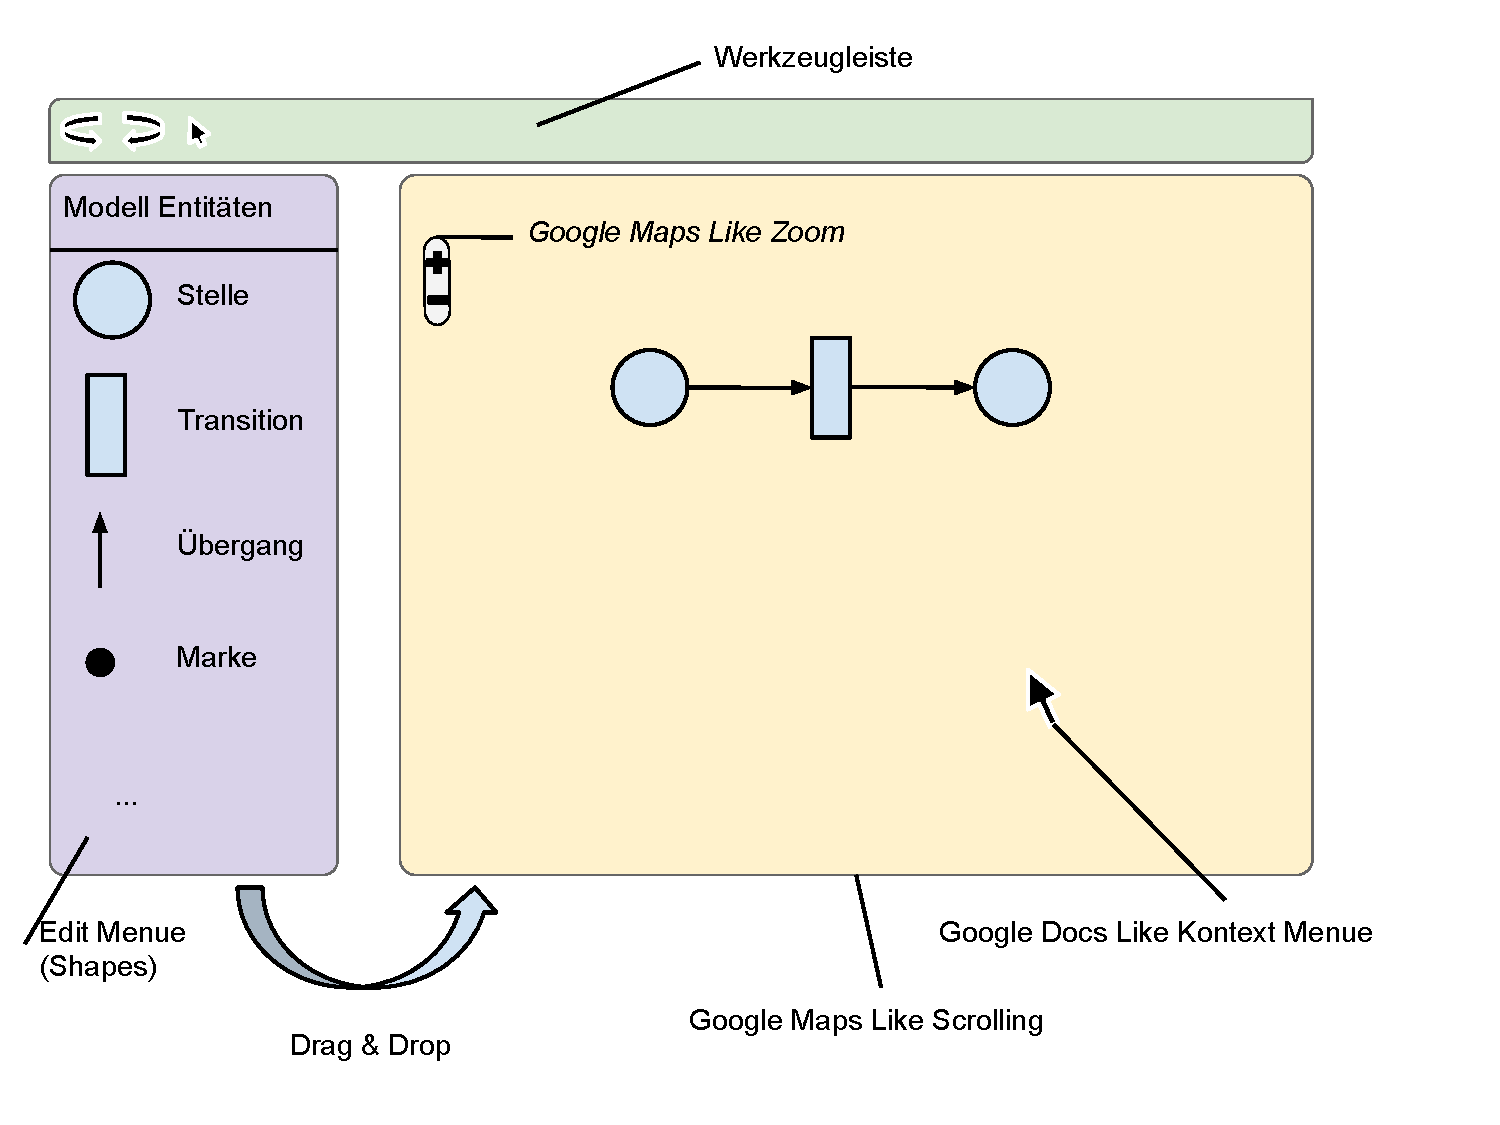
\includegraphics[width=1.0\textwidth]{Figures/Entwurf_GUI.pdf}
  \caption{Entwurf GUI (Beispiel Modell: Petrinetz).}\label{fig.gui}
\end{figure}

\begin{figure}[h!]
  \centering
  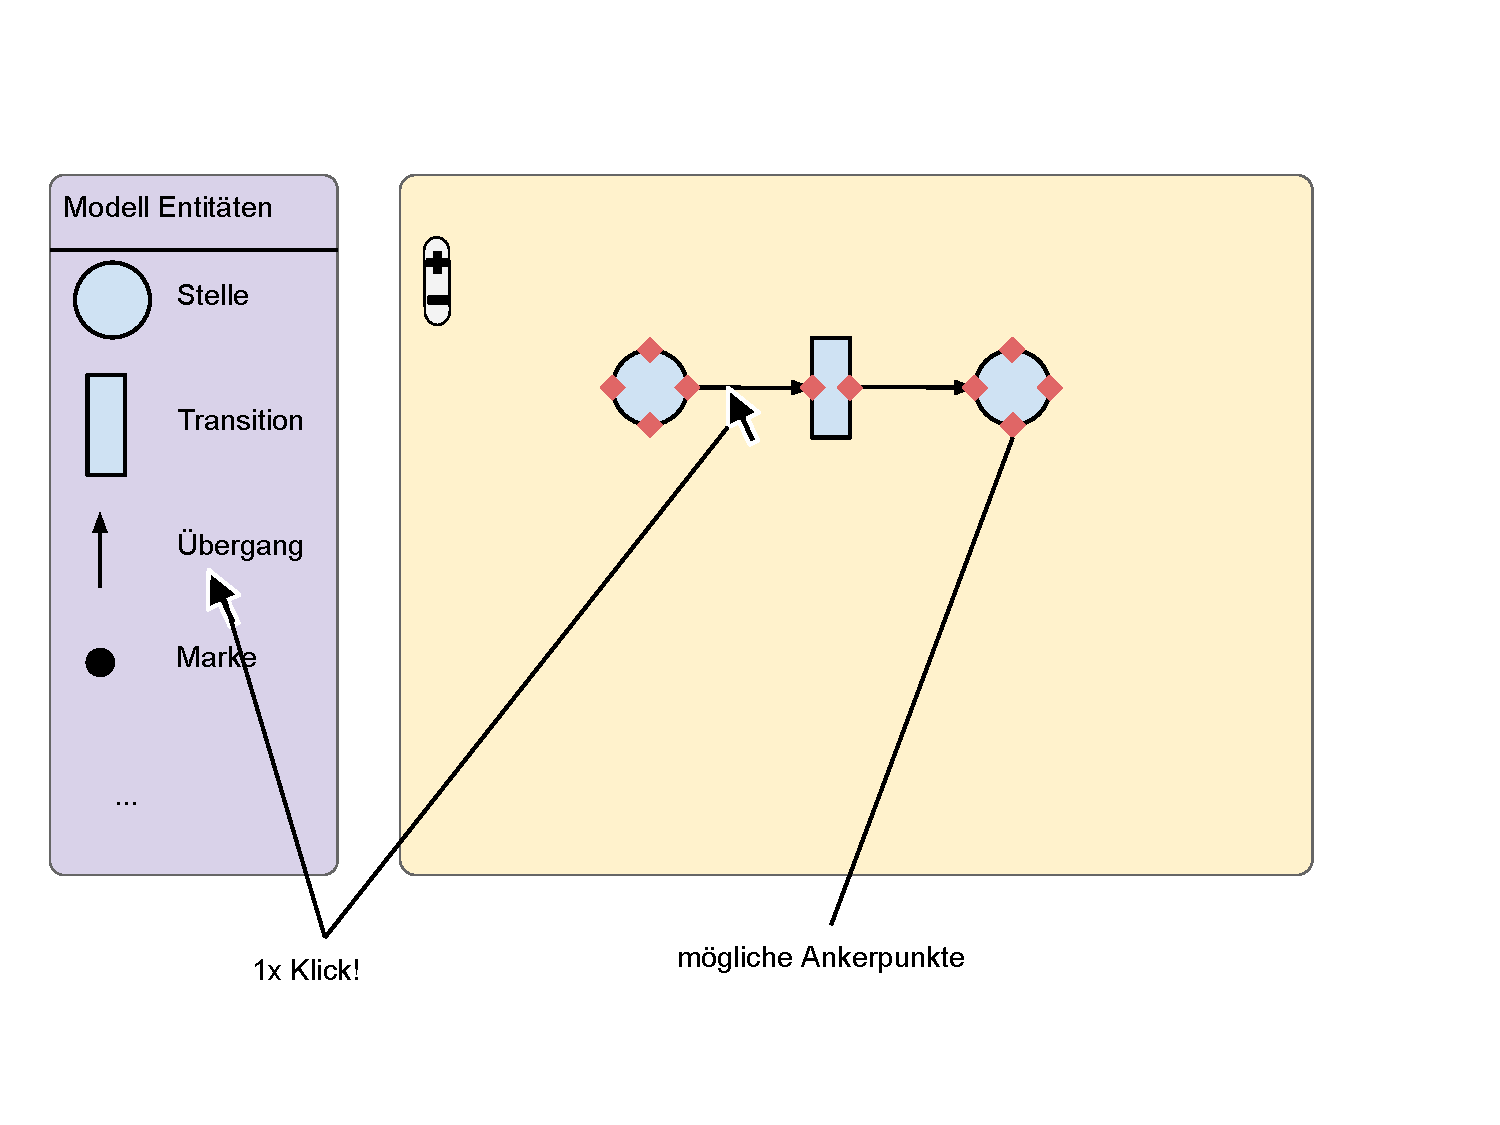
\includegraphics[width=1.0\textwidth]{Figures/Entwurf_GUI_Anker.pdf}
  \caption{Entwurf GUI: Ankerpunkte Auswahl (Beispiel Modell: Petrinetz).}\label{fig.guiAnker}
\end{figure}

\noindent Anforderungen an die Werkzeugleiste die auf Abbildung
\ref{fig.gui} dargestellt wird:

\begin{itemize}
  \item Undo, Redo
  \item Select,  damit kann ein oder mehrere Shapes selektioniert werden
  \item Werkzeuge mit Hotkeys bedienbar (z.B. Undo mit CTRL+Z)
  \item In Modellentitäten: Formen entsprechen der zur Verfügung stehenden Spray Elemente
  \item In Modellentitäten: Die Formen können per Drag and Drop in die Fläche gezogen werden
  \item Optional: Reihenfolge der Elemente bestimmbar (Vordergrund, Hintergrund)
  \item Optional: Speichern, Laden
\end{itemize}


\paragraph{Primitive Shapes}\label{sec.primitivShapes}

Es ist essentiell, dass folgende Shape Basistypen dargestellt werden können,
und ineinander verschachtelbar sind
\citep[siehe Kapitel \emph{The Shape grammar}][]{sprayUser}:

\begin{itemize}
  \item Line
  \item PolyLine
  \item Rectangle
  \item RoundedRectangle
  \item Polygon
  \item Ellipse
  \item Text
  \item Anchor
\end{itemize}

\noindent Neben den visuellen Anforderungen gibt es noch weitere Anforderungen:

\begin{itemize}
  \item Die Texte der Shapes können editierbar sein.
  \item Die Shapes sind per Maus positionierbar, drehbar, beliebig skalierbar, löschbar, bearbeitbar. Dafür werden Bearbeitungspunkte eingeblendet.
  \item Interaktive Verschachtelung von Shapes (Compartments)
    \begin{itemize}
      \item Gruppieren, Entgruppieren
      \item Compartments geben die Größe eines Shapes implizit vor. Ist vorgegeben von Shape-DSL. (z.B. Attribute die beim Klassendiagramm hinzukommen)
    \end{itemize}
  \item Allgemeine Verschachtelung von Shapes (statisch) z.B. bereits verschachtelte Shapes durch DSL-Definition
  \item Eigenes Kontextmenü für Shapes
    \begin{itemize}
      \item Add → new Shapes (für statische Verschachtelung)
      \item Cut
      \item Remove
      \item Copy
      \item Rename (wenn benennbar)
      \item Align
      \item Properties: Anzeige von Eigenschaften
    \end{itemize}
  \item Eigenes Kontextmenü für Connections
    \begin{itemize}
      \item Rename
      \item Remove
      \item Align
      \item Properties: Anzeige von Eigenschaften
    \end{itemize}
  \item Kontextmenüs mit Hotkeys bedienbar (z.B. Add mit Space)
  \item Optional: Spezifische Kontextmenüerweiterung für jede Entity
    \begin{itemize}
      \item z.B. Randdicke oder Hintergrundfarbe bei Ellipse
      \item z.B. Shapeumwandlung von Ellipse in Kreis
    \end{itemize}
  \item Ankerpunkte werden durch die Shape-DSL definiert, Anker sind also vorgegeben
  \item Verbindungen zwischen Ankerpunkten werden vom Benutzer definiert
  \item Bei einfachem Klick auf eine Verbindung (Connection) im Edit Menü erscheinen die möglichen Ankerpunkte als Auswahl. (Siehe Abbildung \ref{fig.guiAnker})
  \item Bei einfachem Klick auf das Shape wird das Shape aktiv und die Bearbeitungspunkte (z.B zum Skalieren) werden angezeigt.
  \item Bei Doppelklick auf das Shape passiert nichts
  \item Bei Doppelklick auf das Label (z.B. Text) wird das Shape aktiv und das Label kann bearbeitet werden.
  \item Defaultwert Label „Name des Shapes“
  \item RapidButton bei onmouseover nur bei aktivem Shape, kann man auswählen welche Optionen zur Verfügung stehen. (Beispiel: bei einer UML-Assoziation kann man diese benennen, linke oder rechte Kardinalität setzen; bei z.B. einer Klasse Methoden, Properties hinzufügen/entfernen/ändern, ...)
  \item Shapes müssen durch „Kasten“ markiert und gruppiert werden können.
  \item Die Styles der Shapes sind dynamisch mit CSS konfigurierbar
\end{itemize}

\paragraph{Shape API}

\begin{itemize}
  \item Connections zwischen allen Shapes müssen möglich sein
  \item Die Shape API muss die DSL interpretieren können und entsprechende Werkzeuge anbieten (z.B. Kreis zeichnen)
  \item Die API muss eine Datenpersistierung anbieten, z.B. wird von der Klasse Kreis mehrere Kreise gezeichnet, müssen die Kreise in einer Datenstruktur festgehalten werden.
  \item Die API muss das Modell gegen die DSL prüfen können und ggf. Fehlermeldungen darstellen.
\end{itemize}

\paragraph{Connections}

Im einfachsten Fall sind Connections Verbindungslinien zwischen
zwei Shapes. Somit bilden Shapes (Knoten) und Connections (Kanten)
eine gerichtete Graphenstruktur.
Prinzipiell können jedoch die Endpunkte der Connections auch aus den gleichen
primitiven Shape-Arten zusammengesetzt werden, um ihre visuelle Bedeutung
klar zu machen.

\begin{itemize}
  \item CDLine
  \item CDPolyLine
  \item CDRectangle
  \item CDRoundedRectangle
  \item CDPolygon
  \item CDEllipse
  \item CDText
\end{itemize}

\paragraph{Compartments}
sind Shapes die zur Laufzeit in ein anderes Shape geschachtelt werden können,
oder auch wieder entfernt werden können. Sie sind auch ein semantischer Teil,
neben Shapes und Connections, und werden somit auch im Modell gespeichert.
Es muss also Unterstützung dafür geben, wärend der Benutzer modelliert, Shapes
verschachteln zu können (via Drag and Drop).


\paragraph{Generalisierbarkeit}
Dadurch, dass sämtlicher Code durch Spray-Generatoren automatisch produziert wird,
ist es nötig, dass das Spray Web Framework keinen „fest verdrahteten“ Code
aufweist, sondern vielmehr sehr generellen Code der mit verschiedensten
Eingaben zurecht kommt.
Beispielsweise ein Petrinetz hat andere Shapes und Validierungsregeln,
als ein Heizungssystem. Die Diagramme unterscheiden sich in Anzahl und
Aufbau der Shapes, Connections, Compartments und Validierungsregeln,
daher soll der Code so generell wie möglich gehalten werden.
(Stichwort Reflections)

\subsection{Nicht-funktionale Anforderungen}

Während funktionale Anforderungen definieren was das System leisten soll,
müssen die Eigenschaften des Systems ebenfalls spezifiziert sein.
Nicht-funktionale Anforderungen werden, wie die funktionalen Anforderungen, im
Systemtest verifiziert und müssen daher messbar sein.
Um nicht-funktionale Anforderungen zu spezifizieren,
dient die ISO 25010 als Checkliste:

\paragraph{Zuverlässigkeit}

\begin{itemize}
  \item Das System ist an mindestens 51 Wochen im Jahr erreichbar.
  \item Bei unbeabsichtigtem Bearbeitungsende (durch Browserabsturz, etc.) soll der zuletzt gespeicherte Systemzustand wiederhergestellt werden.
  \item Systemdaten sollen bei Verlust nach 24 Stunden wiederhergestellt werden können.
\end{itemize}

\paragraph{Benutzbarkeit}

\begin{itemize}
  \item Das System ist nicht barrierefrei optimiert.
  \item Ein Nutzer mit guten Internetkenntnissen hat das System spätestens nach einer Stunde Schulung erlernt, verstanden und kann es selbständig fehlerfrei bedienen.
\end{itemize}

\paragraph{Sicherheit}

\begin{itemize}
  \item Das System muss den unauthorisierten Zugriff auf den Server verhindern.
  \item Das System erlaubt nur registrierten Benutzern den Zugriff.
  \item Das System muss Benutzerdaten vertraulich behandeln.
\end{itemize}

\paragraph{Leistung und Effizienz}

\begin{itemize}
  \item Die Übertragung der Signale vom Client an den Server und zurück ist maximal 1 Sekunde verzögert.
  \item Das System muss in der Lage sein, bei einer Änderung eines Shapes, während einer Sekunde die Validität zu prüfen.
  \item Das System muss in der Lage sein, auch komplexe Shape-Darstellungen, in maximal 10 Sekunden zu rendern.
\end{itemize}

\paragraph{Wartbarkeit}

\begin{itemize}
  \item Alle Modultests sollen automatisiert durchgeführt werden.
  \item Jede Klasse soll testbar sein.
  \item Alle Klassen und alle Methoden sind ausreichend dokumentiert.
  \item McCabe-Mass soll nicht höher sein als 8.
\end{itemize}

\paragraph{Übertragbarkeit}

\begin{itemize}
  \item Die Software ist mit einem Aufwand von maximal einem Tag auf ein System, z.B. Windows Server oder Linux, installierbar.
  \item Die Software ist auf ein anderes System, z.B. Windows Server, anpassbar.
\end{itemize}

\paragraph{Kompatibilität}

\begin{itemize}
  \item Die Software unterstützt alle aktuellen Browser, die auf der WebKit-Engine (Safari, Google Chrome) basieren.
  \item Die Software ist kompatibel mit allen Geräten und Betriebssystemen, die die genannten Browser unterstützen.
\end{itemize}

\paragraph{Funktionale Tauglichkeit}

\begin{itemize}
  \item Mindestens 99.5\% aller Signale werden während einer Bearbeitung eines Shape-Diagramms übertragen.
\end{itemize}



\section{Architektur}

Das Design der Architektur ergibt sich aus den Anforderungen
und wird auf der Architekturskizze Abb. \ref{fig.ComponentOverview}
veranschaulicht.

Der Editor im Browser soll alle Shapes zeichnen,
welche von einer Shape-Definition vorgegeben sind.
Die Shape und Logik-Definitionen (class definitions) im JSON-Format kommen von Spray.
Ein Generator in Spray generiert eine JSON-Datei welche die Regeln enthält.
Der Server liefert diese JSON-Dateien statisch an den Browser aus.
Anhand dieser JSON-Datei generiert die Shape Factory entsprechende Figuren
mit Hilfe des \dd~ Frameworks.

Damit \dd~ auch die Regeln (die vorgeben wie ein valides Modell aussieht) beachtet,
werden diese an \dd~ übergeben.
In \dd~ gibt es Funktionen die bei bestimmten Events aufgerufen werden (Listener-Funktionen). Dazu gehören unter anderem die Policy-Funktionen.
In diesen Funktionen wird überprüft ob die gegebene „Grammatik“ des Modells
verletzt wird. Ist dies der Fall wird die entsprechende Aktion nicht ausgeführt.
Damit der Nutzer eine nicht erlaubte Aktion erkennt,
wird das Cursor Symbol zu einem Stop-Symbol geändert.

Damit in Zukunft auch Kollaboration möglich ist, schickt der Client bei jeder Aktion eine Nachricht via Websocket an den Server.
Die Nachricht an den Server enthält die genaue Beschreibung der Aktion.
Aus dieser Beschreibung kann der Server eine Ecore Modellinstanz pflegen,
diese wird zur Laufzeit als XMI persistiert. Bei jeder Nachricht aktualisiert
der Server die XMI Datei.
Ob die Aktion erlaubt ist wird bereits auf dem Client geprüft und muss deshalb nicht mehr auf dem Server validiert werden.
\\\\

\begin{figure}[h!]
  \centering
  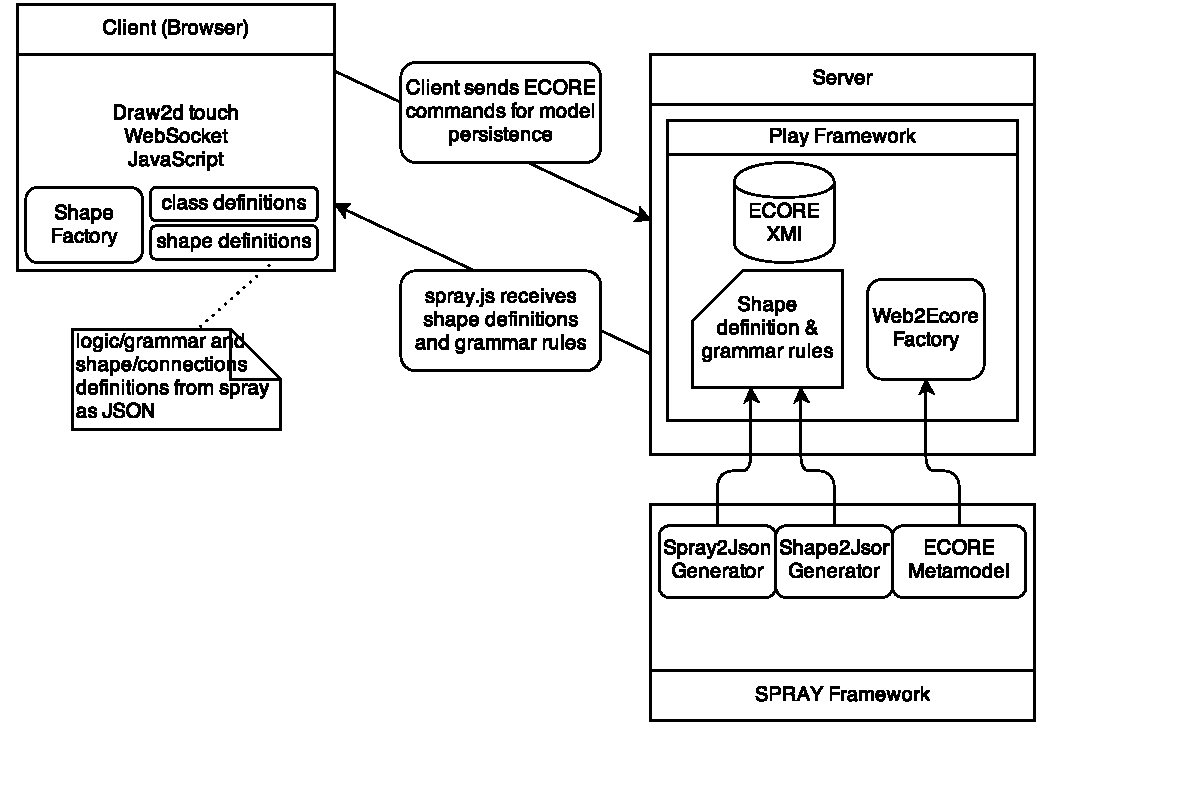
\includegraphics[width=1.0\textwidth]{Figures/ComponentOverview.draw.io.pdf}
  \caption{Übersicht über die wichtigsten Spray Web Komponenten.}
  \label{fig.ComponentOverview}
\end{figure}

\paragraph{spray.js} Dort befindet sich der hauptsächliche Teil des Codes.
Es befindet sich im Repositorium in {\tt server/public/javascripts/spray}.
Da \dd~ nicht allen Anforderungen genügt wird es um entsprechende Klassen erweitert.
Diese \dd~ Klassen werden in {\tt spray2d} gepflegt.
Der {\tt spray2d} Ordner ist somit der Struktur von \dd~ nachempfunden -- Ordner
als auch Namespaces.

Leider musste auch direkt Quellcode von \dd~ angepasst werden, da manche Änderungen
über einfache Klassenvererbung oder Delegation nicht lösbar sind.
Das heißt bei einem Update von \dd~ müssen diese Änderungen unbedingt migriert werden.
